% どうやって解くかの説明

\section{研究の目的}
\begin{frame}
  \frametitle{研究の目的}

  \begin{block}{\textbf{表現力}と\textbf{安全性}を兼ね備えたコード生成言語の構築}
    \begin{itemize}
    \item 表現力: 多段階let挿入,メモ化等の技法を表現
    \item 安全性: 生成されるコードの一定の性質を静的に検査
    \end{itemize}
  \end{block}

  \medskip
  \pause
  % 文字は減らしたほうが良さそう よりってのは何に比べて?
  \begin{block}{本研究: 簡潔で強力なコントロールオペレータに基づくコード生成体系の構築}
    \begin{itemize}
    \item コントロールオペレータ shift0/reset0 を利用し,let挿入などのコード生成技法を表現
    \item 型システムを構築して型安全性を保証
    \end{itemize}
  \end{block}
\end{frame}

\section{研究の内容}

\begin{frame}
  \center
  \huge{表現力を上げ(コードレベルでの多段階let挿入),安全性も保証するためにどうすればよいのか}
\end{frame}

% \subsection{本研究の手法}
% \begin{frame}
%   % 須藤さんの
%   \frametitle{本研究の手法}
%   % \begin{itemize}
%   % \item shift0/reset0 の型システムを単純化; let挿入等に絞る
%   % \item これをコード生成言語の型システムに融合
%   % \item 型システムの安全性を保証: Kameyama+ 2009, Sudo+2014 の手法を利用
%   % \end{itemize}
%   \begin{columns}
%     \begin{column}{1.\textwidth}%% [横幅] 0.2\textwidth = ページ幅の 20 %
%       \center
%       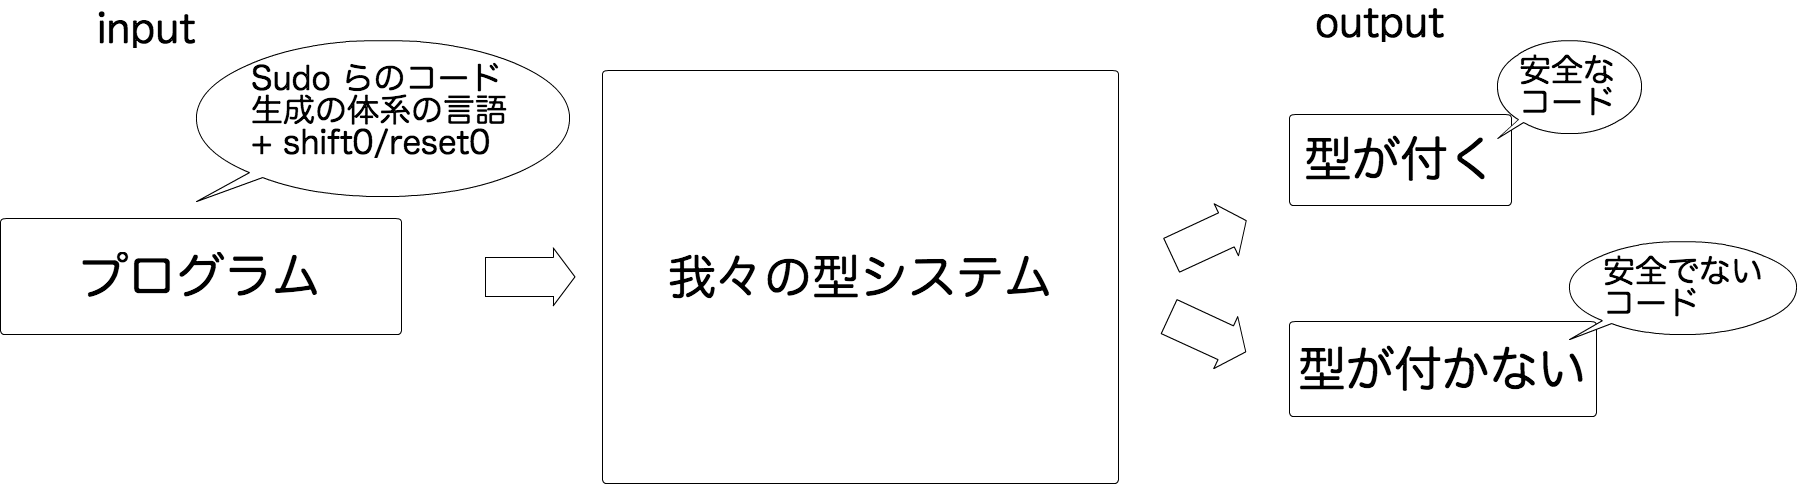
\includegraphics[clip,height=3.2cm]{./img/code_s0r0.png}
%     \end{column}
%   \end{columns}
% \end{frame}

\subsection{コード生成器と生成されるコード}

\begin{frame}
  \center
  \huge{まず表現力について}
\end{frame}

\begin{frame}
  \frametitle{let挿入の実現方法}

  \begin{visibleenv}<1->
    \begin{columns}
      \begin{column}{0.5\textwidth}%% [横幅] 0.2\textwidth = ページ幅の 20 %
        コード生成器
        \begin{align*}
          & \red{\circ}~ \cfordo{x = e1}{e2} \\
          & ~~\red{\circ}~ \cfordo{y = e3}{e4} \\
          & ~~~~~~\caryset{\code{a}}{(x,y)}~ \red{\circ}~ \text{cc}
        \end{align*}
      \end{column}
      $\too$
      \begin{column}{0.5\textwidth}%% [横幅] 0.2\textwidth = ページ幅の 20 %
        生成されるコード
        \begin{align*}
          & \cbra \magenta{\Let ~u' ~= ~\text{cc}' ~\In} \\
          & ~~\fordo{x' = e1'}{e2'} \\
          & ~~~~\fordo{y' = e3'}{e4'} \\
          & ~~~~~~\aryset{a}{x',y'}{u'} \cket
        \end{align*}
      \end{column}
    \end{columns}
  \end{visibleenv}

  \begin{visibleenv}<2>
    \begin{exampleblock}{shift0/reset0の導入}
      $\red{\circ}$ のところに \red{shift0/reset0} を用いることで,多段階let挿入を行う
    \end{exampleblock}
  \end{visibleenv}
\end{frame}

\subsection{多段階let 挿入}

\begin{frame}
  \frametitle{shift0/reset0 によるlet挿入}
  \noindent
  \begin{align*}
    \uncover<3->{\Resetz ~(E[\Shiftz~ k \to e]) ~\leadsto~ e \ksubst{k}{E}}
  \end{align*}

  \noindent

  % \begin{align*}
  %   \text{コード生成器:}~~
  %   & \uncover<4->{\blue{\Resetz}} ~~\cfordo{x = e1}{e2} \\
  %   & ~~\uncover<2-3>{\blue{\Resetz}} ~~\cfordo{y = e3}{e4} \\
  %   & ~~~~\uncover<2->{\blue{\Shiftz}~\blue{k}~\to}~
  %   \magenta{\cLet~u=t~\cIn} \\
  %   & ~~~~~~\uncover<2->{(\blue{\Throw~k}}~(\caryset{a}{(x,y)}{u})
  %   \uncover<2->{)} \\
  %   &   \uncover<3,5->{\blue{k}}
  %   \only<3>{\Leftarrow ~~\cfordo{y = e3}{e4}~[\ ]}
  %   \only<5->{\Leftarrow ~~\cfordo{x = e1}{e2} ~~\cfordo{y = e3}{e4} ~~[\ ]} \\
  %   \text{生成コード:}~~
  %   & \uncover<3,5->{\cbra~}
  %   \only<3>{\fordo{x' = e1'}{e2'}} \only<5->{\magenta{\Let ~u' ~= ~t' ~\In}} \\
  %   & ~~
  %   \only<3>{\magenta{\Let ~u' ~= ~t' ~\In}} \only<5->{\fordo{x' = e1'}{e2'}} \\
  %   & ~~~~\uncover<3,5->{\fordo{y' = e3'}{e4'}} \\
  %   & ~~~~~~\uncover<3,5->{\aryset{a}{x',y'}{u'} ~\cket}
  % \end{align*}

  \begin{align*}
    \scriptsize{\text{コード生成器:}}~~
    & \uncover<2->{\blue{\Resetz}} ~\cfordo{x = e1}{e2} \\
    & ~~~~~~~~~~~\cfordo{y = e3}{e4} \\
    & ~~~~~~~~~~~~\set~a~(x,y)~ \only<1>{cc} \uncover<2->{\blue{\Shiftz~ k \to} \magenta{\cLet~u = cc~\cIn}~ \blue{\Throw~ k}~ u} \\
    % & ~~~~~~~~~~~~~~~~~~~~~~~~~~~~~~~~\uncover<2->{\magenta{\cLet~u = cc~\cIn}~ \blue{\Throw~ k}~ u} \\
    & \uncover<3->{\blue{k} \Leftarrow ~~\cfordo{x = e1}{e2} \\
    & ~~~~~~~~~~~\cfordo{y = e3}{e4} \\
    & ~~~~~~~~~~~~~\caryset{a}{(x,y)}{} [\ ]} \\
    \uncover<4->{\scriptsize{\text{生成コード:}}~~}
    & \uncover<4->{\cbra~}
      \uncover<4->{\magenta{\Let ~u' ~= ~cc' ~\In}} \\
    & ~~~~\uncover<4->{\fordo{x' = e1'}{e2'}} \\
    & ~~~~~~\uncover<4->{\fordo{y' = e3'}{e4'}} \\
    & ~~~~~~~~\uncover<4->{\aryset{a}{x',y'}{u'} ~\cket}
  \end{align*}
\end{frame}


\begin{frame}
  \frametitle{shift0/reset0 による\alert{多段階}let挿入}
  \noindent
  \begin{align*}
    \Resetz ~(E[\Shiftz~ k \to e]) ~\leadsto~ e \ksubst{k}{E}
  \end{align*}

  \noindent
  % \begin{align*}
  %   \text{コード生成器:}~~
  %   & \red{\Resetz} ~~\cfordo{x = e1}{e2} \\
  %   & ~~\blue{\Resetz} ~~\cfordo{y = e3}{e4} \\
  %   & ~~~~\blue{\Shiftz}~\blue{k_2}~\to~
  %     \red{\Shiftz}~\red{k_1}~\to~
  %     \magenta{\cLet~u=t~\cIn} \\
  %   & ~~~~~~\red{\Throw~k_1}~
  %     (\blue{\Throw~k_2}~(\caryset{a}{(x,y)}{u})) \\
  %     % & \red{k_1} \Leftarrow ~~\cfordo{x = e1}{e2}~[\ ] \\
  %     % & \blue{k_2} \Leftarrow ~~\cfordo{y = e3}{e3}~[\ ] \\
  %   \text{生成コード:}~~
  %   & \cbra~\magenta{\Let ~u' ~= ~t' ~\In} \\
  %   & ~~\fordo{x' = e1'}{e2'} \\
  %   & ~~~~\fordo{y' = e3'}{e4'} \\
  %   & ~~~~~~\aryset{a}{x',y'}{u'} ~\cket
  % \end{align*}

  \begin{align*}
    \scriptsize{\text{コード生成器:}}~~
    & \red{\Resetz} ~~\cfordo{x = e1}{e2} \\
    & ~~\blue{\Resetz} ~~\cfordo{y = e3}{e4} \\
    & ~~~~ \caryset{a}{(x,y)}{\blue{\Shiftz~ k_1 \to}~ \magenta{\cLet~ u = cc1~ \cIn~} \blue{\Throw~ k_1}~ u;} \\
    & ~~~~ \set~ b~ (x,y)~ \blue{\Shiftz~ k_1 \to~} \red{\Shiftz~ k_2 \to}~ \\
    & ~~~~~~~~~~~~~~~~~~~~~~~~ \magenta{\cLet~ w = cc2~ \cIn~} \red{\Throw~ k_2} (\blue{\Throw~ k_1}~ w) \\
    % & \red{k_1} \Leftarrow ~~\cfordo{x = e1}{e2}~[\ ] \\
      % & \blue{k_2} \Leftarrow ~~\cfordo{y = e3}{e3}~[\ ] \\
    \uncover<2->{\scriptsize{\text{生成コード:}}~~}
    & \uncover<2->{\cbra~\magenta{\Let ~w' ~= ~cc2' ~\In}} \\
    & \uncover<2->{~~~~\fordo{x' = e1'}{e2'}} \\
    & \uncover<2->{~~~~~~\magenta{\Let ~u' ~= ~cc1' ~\In}} \\
    & \uncover<2->{~~~~~~~~\fordo{y' = e3'}{e4'}} \\
    & \uncover<2->{~~~~~~~~\aryset{a}{x',y'}{u'}} \\
    & \uncover<2->{~~~~~~~~\aryset{b}{x',y'}{w'} ~\cket}
  \end{align*}
\end{frame}

\begin{frame}
  \center
  \huge{次に安全性}
\end{frame}

\begin{frame}
  \center
  \huge{コード生成前の段階で,安全なコードかどうかを判断する}
\end{frame}

% \begin{frame}
%   \center
%   \huge{安全なコードにのみ型をつけるにはどうすればよいか}
% \end{frame}

\subsection{型システム}

\begin{frame}
  \frametitle{環境識別子(EC)を利用したスコープ表現\tiny{[Sudo+2014]}}
  % \begin{center}
  %   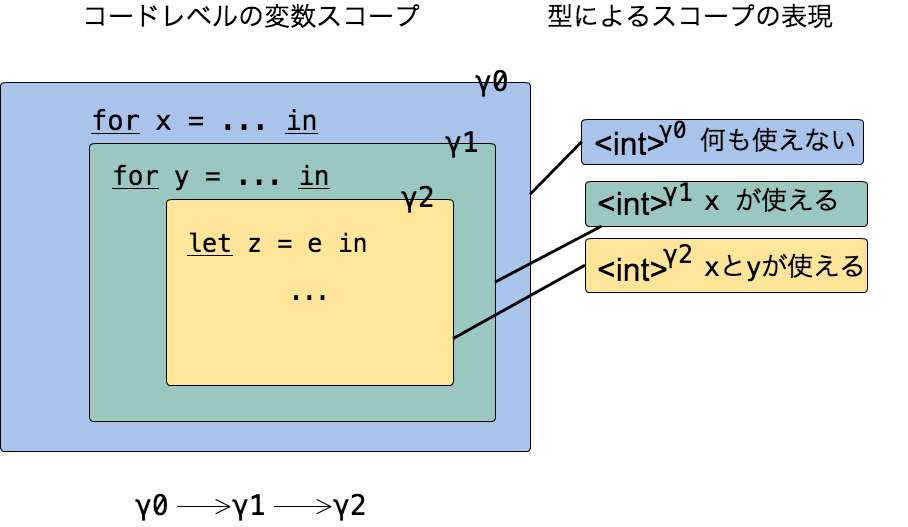
\includegraphics[clip,height=5.7cm]{./img/ec_for.png}
  % \end{center}
  % \begin{flushright}
  %   $\gamma_i ... \text{Refined Environment Classifier}$
  % \end{flushright}

  \newcommand\ml{\multicolumn}
  {\Large
    \begin{tabular}{l|l|l|l|l|l|}
      \cline{2-6}
      \alert{$\mathbf \gamma0$} & \ml{5}{|l|}{$\cfordo{x = e1}{e2}~~~~~~~~~~~~~~~$} \\ \cline{3-5}
                                & \alert{$\mathbf \gamma1$} & \ml{3}{|l|}{$\cfordo{y = e3}{e4}$} & \\ \cline{4-4}
                                &           & \alert{$\mathbf \gamma2$} & \ml{1}{|l|}{$\caryset{a}{(x,y)} cc$} & ~~ & \\ \cline{4-4}
                                &           & \ml{3}{|l|}{\ }    &               \\ \cline{3-5}
                                & \ml{5}{|l|}{~~~~~~~~~~~~~~~~~~ } \\ \cline{2-6}
    \end{tabular}
  }

  \begin{center}
    \begin{tabular}{c|c}
      スコープ & 使えるコード変数 \\ \hline
      \red{$\gamma0$} & なし \\ \hline
      \red{$\gamma1$} & $x$ \\ \hline
      \red{$\gamma2$} & $x, y$
    \end{tabular}\qquad
  \end{center}

\end{frame}

\begin{frame}
  \frametitle{環境識別子(EC)を利用したスコープ表現\tiny{[Sudo+2014]}}
  % 大なり記号はスコープの大きさを表しているのではなく,使える自由変数の集合の大きさを表している
  型システムでコード変数のスコープを表現:

  \center
  \begin{align*}
    & \Gamma = \gamma2 \ord \gamma1,~
      x : \codeTs{\textbf{int}}{\gamma1},~
      y : \codeTs{\textbf{int}}{\gamma2}
  \end{align*}

  \begin{tabular}{c|c}
    $\gamma1$ & $\gamma2$ \\ \hline \hline
    \uncover<1->{$\Gamma ~\vdash~ x : \codeTs{\textbf{int}}{\gamma1}~~ \alert{\text{OK}}$} & \uncover<1->{$\Gamma ~\vdash~ x : \codeTs{\textbf{int}}{\gamma2}~~ \alert{\text{OK}}$} \\ \hline

    \uncover<1->{$\Gamma ~\vdash~ y : \codeTs{\textbf{int}}{\gamma1}~~ \alert{\text{NG}}$} & \uncover<1->{$\Gamma ~\vdash~ y : \codeTs{\textbf{int}}{\gamma2}~~ \alert{\text{OK}}$} \\ \hline

    \uncover<1->{$\Gamma ~\vdash~ x\cPlus y : \codeTs{\textbf{int}}{\gamma1}~~  \alert{\text{NG}}$} & \uncover<1->{$\Gamma ~\vdash~ x\cPlus y : \codeTs{\textbf{int}}{\gamma2}~~  \alert{\text{OK}}$}
  \end{tabular}

  \bigskip

  \begin{uncoverenv}<2->
    コードレベルのラムダ抽象の型付け規則で固有変数条件を利用:

    \[
      \infer[(\gamma_2~\text{is eigen var})]
      {\Gamma \vdash \cfun{x}{e} : \codeTs{t_1\to t_2}{\gamma_1} }
      {\Gamma,~\gamma_2 \ord \gamma_1,~x:\codeTs{t_1}{\gamma_2} \vdash
        e : \codeTs{t_2}{\gamma_2}}
    \]
  \end{uncoverenv}
\end{frame}

\begin{frame}
  \frametitle{環境識別子(EC)を利用したスコープ表現}

  先行研究:
  \begin{itemize}
  \item 局所的なスコープをもつ破壊的変数をもつコード生成の体系に対する(型安全な)型システムの構築
    [Sudo,Kiselyov,Kameyama 2014]
  \item グローバルなスコープをもつ破壊的変数への拡張
    [Kiselyov,Kameyama,Sudo 2016]
  \item[◯] コントロールオペレータには非対応
  \end{itemize}

  \medskip
  \begin{uncoverenv}<2->
    \begin{exampleblock}{問題点:}
      shift0/reset0 などのコントロールオペレータは,スコープの包含関係を逆転させてしまう.
    \end{exampleblock}
  \end{uncoverenv}
\end{frame}

\begin{frame}
  \center
  \huge{環境識別子(EC)の問題点}
\end{frame}


% \begin{frame}
%   \frametitle{環境識別子(EC)の問題点}
%   % sudo らの研究の EC を素朴に適用させると問題があるということ言うスライド
%   %ここに,forループとshift0/reset0 の例を再掲する.
%   %もとのスライドの 24ページの絵をかく.

%   \newcommand\ml{\multicolumn}

%   \begin{uncoverenv}<1->
%     コード生成器:\\
%     \begin{tabular}{l|l|l|l|l|l|}
%       \cline{2-6}
%       & \ml{5}{|l|}{\cfordo{x = e1}{e2}~~~~~~~~~~~~~~~} \\ \cline{3-5}
%       & \footnotesize{\alert{$\mathbf \gamma0$}} & \ml{3}{|l|}{\Resetz~ \cfordo{y = e3}{e4}} & \\ \cline{4-4}
%       &           & \footnotesize{\alert{$\mathbf \gamma1$}} & \ml{1}{|l|}{\caryset{a}{(x,y)}{\Shiftz~ k $\to$ \footnotesize{\alert{$\mathbf \gamma2$}} {\large $\mid$} \magenta{\cLet~ u = cc \cIn}~ \footnotesize{\alert{$\mathbf \gamma3$}} {\large  $\mid$} \Throw~ k u}} & ~~ & \\ \cline{4-4}
%       &           & \ml{3}{|l|}{\ }    &               \\ \cline{3-5}
%       & \ml{5}{|l|}{~~~~~~~~~~~~~~~~~~ } \\ \cline{2-6}
%     \end{tabular}
%   \end{uncoverenv}

%   \begin{uncoverenv}<2>
%     生成コード:\\
%     \begin{tabular}{l|l|l|l|l|l|l|l|l|l|l|l|l|}
%       \cline{2-10}
%       & \ml{9}{|l|}{$\fordo{x' = e1'}{e2'}$~~~~~~~~~~~~~~~} \\ \cline{3-9}
%       & \footnotesize{\alert{$\mathbf \gamma0$}} & \ml{7}{|l|}{\magenta{$\Let~ u' = cc' ~ \In$}~} & \\ \cline{4-8}
%       & & \footnotesize{\alert{$\mathbf \gamma2$}} & \ml{5}{|l|}{$\fordo{y' = e3'}{e4'}$}  & & \\ \cline{5-7}
%       & & & \footnotesize{\alert{$\mathbf \gamma3$}} & \ml{3}{|l|}{\ }     &   &  &       \\ \cline{6-6}
%       & & & & \footnotesize{\alert{$\mathbf \gamma1$}} & \ml{1}{|l|}{$\aryset{a}{(x',y')}{u'}$} & & &  &  \\ \cline{6-6}
%       & & & & \ml{3}{|l|}{\ }  &   &   &           \\ \cline{5-7}
%       & & & \ml{5}{|l|}{\ } &  &               \\ \cline{4-8}
%       & & \ml{7}{|l|}{\ }  & \\ \cline{3-9}
%       & \ml{9}{|l|}{~~~~~~~ } \\ \cline{2-10}
%     \end{tabular}
%   \end{uncoverenv}

% \end{frame}

% \begin{frame}
%   \frametitle{環境識別子(EC)の問題点}
%   \center
%   コード生成器:
%   \begin{tabular}{c|c}
%     スコープ & 使えるコード変数 \\ \hline
%     \red{$\gamma0$} & x \\ \hline
%     \red{$\gamma1$} & x,y \\ \hline
%     \red{$\gamma2$} & x,y \\ \hline
%     \red{$\gamma3$} & x,y,u \\
%   \end{tabular}\qquad

%   \bigskip

%   生成コード:
%   \begin{tabular}{c|c}
%     スコープ & 使えるコード変数 \\ \hline
%     \red{$\gamma0$} & x \\ \hline
%     \red{$\gamma1$} & x,u \\ \hline
%     \red{$\gamma2$} & x,y,u \\ \hline
%     \red{$\gamma3$} & x,y,u \\
%   \end{tabular}\qquad

%   \begin{itemize}
%   \item 生成前と生成後の$\gamma1$ と $\gamma2$ の間には順序関係がない
%   \item $\gamma1$ $\cup$ $\gamma2$ = $\gamma3$
%   \end{itemize}
% \end{frame}

\begin{frame}
  \frametitle{コード生成前・後でスコープの包含関係が逆転}
  % sudo らの研究の EC を素朴に適用させると問題があるということ言うスライド
  %ここに,forループとshift0/reset0 の例を再掲する.
  %もとのスライドの 24ページの絵をかく.

  \newcommand\ml{\multicolumn}

  \begin{uncoverenv}<1->
    コード生成器:
    \footnotesize
    \begin{tabular}{l|l|l|l|l|l|l|l|l|l|l|l|l|}
      \cline{2-10}
      & \ml{9}{|l|}{$\cfordo{x = e1}{e2}$~~~~~~~~~~~~~~~} \\ \cline{3-9}
      & \footnotesize{\alert{$\mathbf \gamma0$}} & \ml{7}{|l|}{$\Resetz~ \cfordo{y = e3}{e4}$~} & \\ \cline{4-8}
      & & \footnotesize{\alert{$\mathbf \gamma1$}} & \ml{5}{|l|}{$\Shiftz~ k \to \magenta{\cLet~ u = cc ~ \In}$}  & & \\ \cline{5-7}
      & & & \footnotesize{\alert{$\mathbf \gamma2$}} & \ml{3}{|l|}{$\Throw~ k$}     &   &  &       \\ \cline{6-6}
      & & & & \footnotesize{\alert{$\mathbf \gamma3$}} & \ml{1}{|l|}{$\caryset{a}{(x,y)}{u}$} & & &  &  \\ \cline{6-6}
      & & & & \ml{3}{|l|}{\ }  &   &   &           \\ \cline{5-7}
      & & & \ml{5}{|l|}{\ } &  &               \\ \cline{4-8}
      & & \ml{7}{|l|}{\ }  & \\ \cline{3-9}
      & \ml{9}{|l|}{~~~~~~~ } \\ \cline{2-10}
    \end{tabular}
  \end{uncoverenv}

  \bigskip

  \begin{uncoverenv}<2>
    生成コード:~~
    \footnotesize
    \begin{tabular}{l|l|l|l|l|l|l|l|l|l|l|l|l|}
      \cline{2-10}
      & \ml{9}{|l|}{$\fordo{x' = e1'}{e2'}$~~~~~~~~~~~~~~~} \\ \cline{3-9}
      & \footnotesize{\alert{$\mathbf \gamma0$}} & \ml{7}{|l|}{\magenta{$\Let~ u' = cc' ~ \In$}~} & \\ \cline{4-8}
      & & \footnotesize{\alert{$\mathbf \gamma2$}} & \ml{5}{|l|}{$\fordo{y' = e3'}{e4'}$}  & & \\ \cline{5-7}
      & & & \footnotesize{\alert{$\mathbf \gamma1$}} & \ml{3}{|l|}{\ }     &   &  &       \\ \cline{6-6}
      & & & & \footnotesize{\alert{$\mathbf \gamma3$}} & \ml{1}{|l|}{$\aryset{a}{(x',y')}{u'}$} & & &  &  \\ \cline{6-6}
      & & & & \ml{3}{|l|}{\ }  &   &   &           \\ \cline{5-7}
      & & & \ml{5}{|l|}{\ } &  &               \\ \cline{4-8}
      & & \ml{7}{|l|}{\ }  & \\ \cline{3-9}
      & \ml{9}{|l|}{~~~~~~~ } \\ \cline{2-10}
    \end{tabular}
  \end{uncoverenv}
\end{frame}

\begin{frame}
  \frametitle{コード生成前・後でスコープの包含関係が逆転}
  \center
  コード生成器:
  \begin{tabular}{c|c}
    スコープ & 使えるコード変数 \\ \hline
    \red{$\gamma0$} & $x$ \\ \hline
    \red{$\gamma1$} & \uncover<1->{$x, y$} \uncover<2->{$\Rightarrow$ \red{$x, y, u$}} \\ \hline
    \red{$\gamma2$} & \uncover<1->{$x, y, u$} \uncover<2->{$\Rightarrow$ \red{$x ,u$}}\\ \hline
    \red{$\gamma3$} & $x, y, u$ \\
  \end{tabular}\qquad

  \bigskip

  生成コード:
  \begin{tabular}{c|c}
    スコープ & 使えるコード変数 \\ \hline
    \red{$\gamma0$} & $x'$ \\ \hline
    \red{$\gamma2$} & $x', u'$ \\ \hline
    \red{$\gamma1$} & $x', y', u'$ \\ \hline
    \red{$\gamma3$} & $x', y', u'$ \\
  \end{tabular}\qquad

  \begin{itemize}
  \item 生成前と生成後の$\gamma1$ と $\gamma2$ の間には順序関係がない
  % \item $\gamma1$ $\cup$ $\gamma2$ = $\gamma3$
  \end{itemize}
\end{frame}


% \begin{frame}
%   \frametitle{本研究での解決策}

%   3つのアイディア:
%   \begin{itemize}
%   \item 包含関係にないEC
%   \item ジョイン演算子
%   \item EC に関する多相性
%   \end{itemize}

% \end{frame}

\begin{frame}
  \center
  \huge{解決策}
\end{frame}

\begin{frame}
  \frametitle{本研究の解決策}
  \flushleft
  
\includegraphics[clip,height=3cm]{./img/ecgraph.png}
  \begin{itemize}
  \item<2-> $\gamma1$ のコードレベル変数は $\gamma2$ では使えない
  \item<2-> $\gamma2$ のコードレベル変数は $\gamma1$ では使えない
  \item<3->[$\Rightarrow$] \red{$\gamma1$ と $\gamma2$ の間に順序を付けない}
  \end{itemize}

  \begin{itemize}
  \item<4-> $\gamma1, \gamma2$ のコードレベル変数は $\gamma3$ で使える
  \item<5->[$\Rightarrow$] \red{Sudoらの体系に $\cup$ (ユニオン) を追加} % ジョイン
  \end{itemize}
\end{frame}

\begin{frame}[fragile]
  \frametitle{コード生成+shift0/reset0 の型システム\small{ (の一部)}}
  reset0:
  \[
    \infer{\Gamma \vdash \resetz{e} : \codeTs{t}{\gamma} ~;~ \sigma}
    {\Gamma \vdash e : \codeTs{t}{\gamma} ~;~ \codeTs{t}{\gamma}, \sigma}
  \]

  shift0:
  \[
    \infer{\Gamma \vdash \shiftz{k}{e} : \codeTs{t1}{\red{\gamma1}} ~;~ \codeTs{t0}{\gamma0},\sigma}
    {\Gamma,~k:\contT{\codeTs{t1}{\gamma1}}{\codeTs{t0}{\gamma0}}
      \vdash e : \codeTs{t0}{\red{\gamma0}} ~;~ \sigma
      & \Gamma \models \gamma1 \ord \gamma0
    }
  \]

  throw:
  \[
    \infer
    {\Gamma,~k:\contT{\codeTs{t1}{\gamma1}}{\codeTs{t0}{\gamma0}}
      \vdash \throw{k}{v} : \codeTs{t0}{\gamma2} ~;~ \sigma}
    {\Gamma
      \vdash v : \codeTs{t1}{\red{\gamma1 \cup \gamma2}} ~;~ \sigma
      & \Gamma \models \gamma2 \ord \gamma0
    }
  \]
\end{frame}


%%% Local Variables:
%%% mode: japanese-latex
%%% TeX-master: "slide"
%%% End:
